% AA vers. 9.0, LaTeX class for Astronomy & Astrophysics
% demonstration file
%                                                       (c) EDP Sciences
%-----------------------------------------------------------------------
\documentclass{aa}  
\usepackage{graphicx}
%%%%%%%%%%%%%%%%%%%%%%%%%%%%%%%%%%%%%%%%
\usepackage{txfonts}
%%%%%%%%%%%%%%%%%%%%%%%%%%%%%%%%%%%%%%%%
%\usepackage[options]{hyperref}
% To add links in your PDF file, use the package "hyperref"
% with options according to your LaTeX or PDFLaTeX drivers.

\begin{document} 


   \title{Select stable radio sources to define ICRF}

   \author{N. Liu}

   \institute{School of Astronomy and Space Science, Nanjing University,
               210023 Nanjing, PR China\\
              \email{liuniu@smail.nju.edu.cn}
             }

%   \date{Received September 15, 1996; accepted March 16, 1997}
 
  \abstract
  % context heading (optional)
  % {} leave it empty if necessary  
   {}
  % aims heading (mandatory)
   {}
  % methods heading (mandatory)
   {}
  % results heading (mandatory)
   {}
  % conclusions heading (optional), leave it empty if necessary 
   {}

   \keywords{
                astrometry --
                reference systems:
                inteferometric
               }

   \maketitle
   
%%2016, Mar 28
%%I change my stuctures and finish it by Apirl 4. I promise!!
%1. Introduction
%2. Data and pre-selection
%3. Selection considerations
%3.1 On the axial stability
%3.2 On the sky distribution
%3.3 On the two aspects above both
%4. Conclusion      
%
%-------------------------------------------------------------------
\section{Introduction}

In 1994 the International Astronomical Union (IAU) recommended the adoption of a celestial reference system, realized by the precise coordinates of a set of extra-galactic radio sources observed with the Very Long Baseline Interferometry (VLBI).

%The previous studies usually select stable sources by investigating three aspects of the observation data: observation history; positional stability as seen from coordinate time series; source structure. In this study we only consider the statistical characteristics of coordinate time series.

%For clarity, in the following sections, the 212 and 295 ICRF defining sources will be referred to as "ICRF1" and "ICRF2" respectively. 
%--------------------------------------------------------------------
%\section{Data and Selection schemes}
%\subsection{Data and Pre-selection}
\section{Data and Pre-selection}
The Paris Observatory IVS analysis center provided a set of coordinate time series for 3778 sources 
%over 1979-2016
\footnote{http://ivsopar.obspm.fr/radiosources/index.php} obtained from VLBI solution,
%cited to S. Lambert 2013 
in which both the 212 ICRF and  295 ICRF2 defining sources are included. We extract the data between August 1979 and January 2016 from the data set, and select the suitable defining sources entirely based on this set of time series. 
%, on which our study is entirely based. 
%For convenience, we will refer these 3778 sources as "OPA3778", 
Figure 
%citation to figure
are statical histograms of length of the observation span and amount of the observational session for a individual source, displaying the observational history of the 3778 sources. To exclude the sources with a poor observation or known extended structure, a pre-selection is appropriate. 

First, 39 special handling sources with large structure\citep[see][]{2009ITN....35....1M} was excluded. Then a pre-selection algorithm is applied to the other 3739 sources for both $\alpha$ and $\delta$ coordinate, as shown below.
	\begin{enumerate}
      \item Length of observation span longer than 5 years.
      \item Number of observation sessions larger than 20.
	  \item Length of successive years with a poor observation less than 10 years. A year with a poor observation here means that within this year the number of observation sessions is less than three.
	  %The length of successive years with no observations less than 3 year for the annual coordinate time series.
   \end{enumerate}

Criterion 1 and 2 promise that the source was well observed over the data span to ensure a reliable linear fitting to both $\alpha$ and $\delta$ coordinate, while criterion 3 represents the continuity of time series. These criteria is artificial, and is determined after trying different values. The aim here is to pick out a set of candidate sources, which means that the criteria cannot be too strict. 10 years in criterion 3 seems to be loose, especially criterion 3, however there are still 
%number
ICRF2 defining sources fail to pass this criterion. 

After Pre-selection, 
%No
sources is considered as candidates, among which
%No
are ICRF2 defining sources.
%To study the statistical stability, we also computed the yearly mean coordinates weighed according to the corresponding uncertainties, based on at least three sessions. Otherwise, the yearly point is considered as null. Then we obtain the time series of the annual coordinates.

%We keep the 295 ICRF defining sources, and apply the selection algorithm to the other 3483 non-defining sources. Before the selection, we exclude the 39 special handling sources with large structure\citep[see][]{2009ITN....35....1M}. To study the statistical stability, we also computed the yearly mean coordinates, weighed according to the corresponding uncertainties, consisting a time series of the annual coordinates. Within the windows, the number of sessions is large than 3. Otherwise, the yearly point is considered as zero with large uncertainty.

%We only consider the sources with a long and continue observational history as candidates, so a preselection was done, based on the following criteria for both $\alpha$ and $\delta$ coordinate.  
%	\begin{enumerate}
%      \item The length of observation span longer than 5 years, and the number of observation sessions larger than 20 for the session coordinate time series.
%	  \item The length of successive years with no observations less than 3 year for the annual coordinate time series.
%   \end{enumerate}

%The observation history are shown in \ref{NumSes} and \ref{ObsSpn}. 463 sources are kept in our candidate list. These include 278 ICRF2 defining sources, and 185 non-defining sources. 7 ICRF2 defining sources fail to pass criteria(1): 
%0458+138
%1448-648
%1554-643
%1611-710
%1633-810
%1824-582
%2344-514,
%while another 10 for criteria(2):
%0007+106
%0342+147
%0358+210
%0949+354
%1030+074
%1049+215
%1443-162
%1456+044
%1508+572
%1745+624.


%Here we select stable sources in the following two steps. 
%
%A first selection is based on the following criteria. For the session coordinate time series,
%	\begin{enumerate}
%      \item The length of observation span is longer than 5 years.
%      \item The number of observation sessions is larger than 20.
%%For the session coordinate time series.
%%	  \item The number of successive zero-points is less than 3.\\
%%for the annual coordinate time series
%   \end{enumerate}
%   And for the annual coordinate time series, the number of successive zero-points is less than 3. 
%   
%This first selection keeps 320 sources well observed, plus the 295 defining sources, consisting a preselected ensemble of 615 candidates .

%%%%%%%%%%%%%%%%%%%%%%%%%%%%%%%%
%Rewritten, Mar 31


%
%-----------------------------------------------------------------
%Figures
%   \begin{figure}
%   \centering
%   \includegraphics[width=\hsize]{figures/Number_of_sessions.ps}
%      \caption{
%      Number of sessions in which a given source is observed. The bar above 1000 means that these sources are observed in more than 1000 sessions.
%              }
%         \label{NumSes}
%   \end{figure}
   
%   \begin{figure}
%   \centering
%   \includegraphics[width=\hsize]{figures/Observation_span.ps}
%      \caption{
%      The length of observation history.
%              }
%         \label{ObsSpn}
%   \end{figure}
   
%	\begin{figure}
%   \centering
%   \includegraphics[width=\hsize]{figures/Observation_history.ps}
%      \caption{
%      Observation history of 642 sources, including 295 ICRF2 defining sources($red$) and 347 non-defining sources($blue$).
%              }
%         \label{ObsHis}
%   \end{figure}
   
%\subsection{Selecting stable sources}
%Although we assume that the radio sources has no proper motion because of their extremely far distances, the time series of coordinate however show "apparent proper motion". The reason for this phenomenon is complex, i.e., an immediate rejection of jet or the extend structure. The "apparent proper motion" of some sources are too large to be considered as unstable. Hence we mainly consider the linear drift of $\alpha\cos\delta$ and $\delta$ (least squares estimation) as the estimators, and we call it "proper motion" of source just for convenience in this work. 

Some previous studies show that quality of early VLBI data is much worse compared to that of the later, and the data before 1990.0 must be used with much caution. This is the reason that some studies on selecting source are based on the coordinate time series only after 1990.0. To keep the database completely, we use all the observation data over 1979.0-2016.0, but in least squares estimation, the weight of a single session is not corresponded to its uncertainty. We divide the time series into three observation span : 1979.0$\sim$1990.0; 1990.0$\sim$2009.0; 2009.0$\sim$2016.0. And the average weight is used as weight of session points within the corresponding observation span. The normal equation of estimation is then different from the usual one, given by (\ref{eq:normal}).
\begin{equation}
\label{eq:normal}
\vec{x}  = N^{-1}_1 \vec{y_1} + N^{-1}_2 \vec{y_2} + N^{-1}_3 \vec{y_3}
\end{equation} 
where $N_1$, $N_2$, $N_3$ represent the normal matrix of the three observation span respectively, and  $y_1$, $y_2$, $y_3$ the corresponding right function.
% term "right function" need be verified

In addition, we also computed the Allan standard deviation of a one-year sampling time, which is generated by using a one-year-window weighed average.

Figure(to be plotted ) Show that the sources with tiny apparent proper motion mainly locate on the northern hemisphere, which means if some criteria on apparent proper motion is applied to all the candidates a large part of southern sources will be ruled out, causing the celestial frame uniform. IERS 2009
%(citation to be added in future)
introduces a method to avoid the problem, in which sources are binned into 6 intervals of declination by four nodes so that each interval has approximately the same number of sources. Here another way of binning is implemented to ensure that each intervals has  the equal spherical area, and the corresponding nodes are $-30\deg$, $0\deg$ and $30\deg$. 
%\deg seems to not work in this environment
The number of sources in intervals are .
%re-calculate 
%And some sources with huge apparent proper motion are not excepted to be defining, it is better to do a second pre-selection .
A rank index based on apparent proper motion can be given, normalized to 100, which the larger it is, the less possible the corresponding sources will be selected as the defining. 
%%it's rude to determine such a criteria
%We keep the sources with rank index less than 60, 70, 80
%%It is questionable, because I think it is better to simulate. 
%and obtain three sets of sources, 
%% the number of sources
%respectively. The mean declinations are 
%Again, to be filled 
%. And the sources sky distribution and statics are shown.
%plot
%figure


%To obtain a stable frame, 


%On the basis of the session coordinate time series, we derive 
%	\begin{enumerate}
%      \item the linear drift of $\alpha\cos\delta$ and $\delta$(least squares estimation);
%      \item the standard deviation of source position referred to its global average.
%   \end{enumerate}
%      
%With the annual coordinate time series, we derive the Allan standard deviation for a one-year sampling time.

The stability of reference frame can be assessed by fitting the one-order spherical harmonics coefficients of rotation to the apparent proper motion, in which the equations are given below.
% (citation.):
\begin{eqnarray}
      \mu_{\alpha}\cos\delta & = 
%                             & -d_1\sin\alpha + d_2\cos\alpha \\
                                & +r_1\cos\alpha\sin\delta +r_2\sin\alpha\sin\delta -r_3\cos\delta \\
      \mu_{\delta}           & = 
%                             & -d_1\cos\alpha\sin\delta -d_2\sin\alpha\sin\delta +d_3\cos\delta 
      						    & +r_1\sin\alpha - r_2\cos\alpha;
   \end{eqnarray}
The total rotation of reference frame can be given by $r = \sqrt{\sum p_ir_i^2 }$, where $p_i = (1/\sigma_{1}^2)/(\sum 1/\sigma_{i}^2)$. 


%-----------------------------------------------------------------
\section{Assessment of reference frame}
\subsection{Axis stability of reference frame}

%%To estimate the systematic effect of reference frame, we estimate the spherical harmonics by fitting to the linear drifts of $\mu_{\alpha}\cos\delta$ and $\mu_{\delta}$, which are considered as the proper motion of sources. The equations are developed by (citation.):
%\begin{eqnarray}
%      \mu_{\alpha}\cos\delta & = 
%%                             & -d_1\sin\alpha + d_2\cos\alpha \\
%                                & +r_1\cos\alpha\sin\delta +r_2\sin\alpha\sin\delta -r_3\cos\delta \\
%      \mu_{\delta}           & = 
%%                             & -d_1\cos\alpha\sin\delta -d_2\sin\alpha\sin\delta +d_3\cos\delta 
%      						    & +r_1\sin\alpha - r_2\cos\alpha;
%   \end{eqnarray}
%
%   where ($r_1$,$r_2$,$r_3$) is the three coordinate part of global rotation.
%-----------------------------------------------------------------
%\subsection{Uniform of sky distribution of selected sources}
\subsection{Uniform of sky distribution of selected sources}


%-----------------------------------------------------------------
\section{Conclusions}

   \begin{enumerate}
      \item 
      \item 
      \item 
   \end{enumerate}
%-----------------------------------------------------------------

\begin{acknowledgements}
      
\end{acknowledgements}

\bibliographystyle{aa}
%\bibliography{bibtex/aa.bib}
\bibliography{bibtex/aa}
\end{document}
